\documentclass{beamer}

%===============================================================%
\mode<presentation> %use <handout> for handout mode
{
\usetheme[compress, icclabt, numbers]{icclab}

\usefonttheme[onlymath]{serif}
	% \useoutertheme{infolines}
\setbeamercovered{transparent}
}

\usepackage[english]{babel}
\beamerdefaultoverlayspecification{<+->}

\usepackage{mathptmx}
\usepackage{helvet}
\usepackage{courier}
\usepackage[T1]{fontenc}
\usepackage{trajan}
%===============================================================%

\title[BGP-Primer]
{Test Presentation}

\subtitle
{a brief primer on ICCLab}

\author[Harsh]{Piyush Harsh}
\institute
{
  Institute of Applied Information Technology
}

\date[04.10.2014]
{Apr. 10, 2014}

\subject{ICCLab:Internal}


\begin{document}

% Comment out the following to remove the header & footer from the title page
\thispagestyle{empty} 

\begin{frame}
 \titlepage
\end{frame}

\begin{frame}<beamer>
  \frametitle{Outline}
  \tableofcontents
\end{frame}

\section{Introduction}

%\subsection{you can add subsection}

\begin{frame}{Things I will say}

I will tell you...

    \begin{itemize}
    \item things,
    \item stuffs,
    \item and \alert{others}.
    \end{itemize}

\end{frame}

\section{Simple Stuffs}

\subsection{Blocks}

\begin{frame}{Say it with Blocks}

\begin{block}<+->{Block} 
This is a block environment.
\end{block}

\begin{example}
This is an example block environment.
\end{example}

 \begin{alertblock}{Alert Block}
This is an alert block environment.
\end{alertblock}

\end{frame}

\subsection{Equations}

\begin{frame}{Say it with Equations}

\begin{equation}
f(x) = \frac{1}{{\sigma \sqrt {2\pi } }}e^{{{ - \left( {x - \mu } \right)^2 } \mathord{\left/ {\vphantom {{ - \left( {x - \mu } \right)^2 } {2\sigma ^2 }}} \right. \kern-\nulldelimiterspace} {2\sigma ^2 }}}
\end{equation}

  \vspace*{.5cm}
You can put equations into block environment.
  \vspace*{.5cm}

\begin{block}<+->{Gaussian Distribution}
\begin{equation}
f(x) = \frac{1}{{\sigma \sqrt {2\pi } }}e^{{{ - \left( {x - \mu } \right)^2 } \mathord{\left/ {\vphantom {{ - \left( {x - \mu } \right)^2 } {2\sigma ^2 }}} \right. \kern-\nulldelimiterspace} {2\sigma ^2 }}}	
\end{equation}
\end{block}

\end{frame}

\section{Advanced Stuffs}

\subsection{Figure}

\begin{frame}{Say it with Figures}

    \begin{figure}
      \scalebox{0.7}
      {
        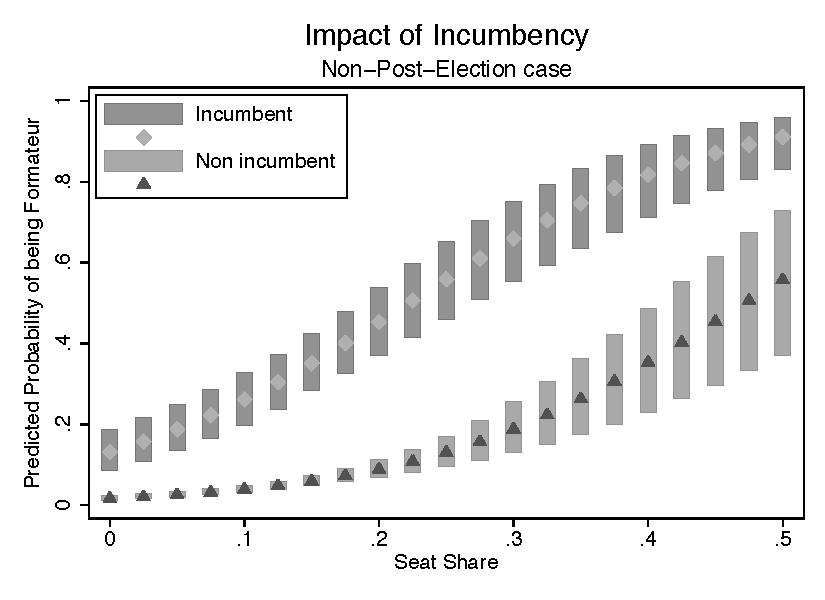
\includegraphics{examplefig}
      }
    \end{figure}

\end{frame}

\subsection{Tables}

\begin{frame}{Say it with Tables}

%------- Begin LaTeX code -------%

{\footnotesize 
\def\sep{0.5em}
\def\fns{\footnotesize}
\def\onepc{$^{\ast\ast}$} \def\fivepc{$^{\ast}$}
\def\tenpc{$^{\dag}$}
\def\legend{\multicolumn{3}{l}{\footnotesize{Significance levels
:\hspace{1em} $\dag$ : 10\% \hspace{1em}
$\ast$ : 5\% \hspace{1em} $\ast\ast$ : 1\% \normalsize}}}
\begin{table}[htbp]\centering
 \caption{Estimation results : regress
\label{tabresult regress}}
\begin{tabular}{l r @{} l }\hline\hline 
\multicolumn{1}{c}
{\textbf{Variable}}
 & \textbf{Coefficient} \\& \fns{(Std. Err.)} \\ \hline
mpg &  -292.434&\onepc \\ & \fns{(60.227)} &\\[\sep]
foreign & 1023.208& \\ & \fns{(866.086)} &\\[\sep]
Intercept & 10586.485&\onepc \\ & \fns{(1555.745)} &\\[\sep]
\hline
\multicolumn{3}{c}{}\\
\hline N & \multicolumn{2}{c}{69}\\
R$^{2}$ & \multicolumn{2}{c}{0.267}\\
F $ _{(3,65)}$ & \multicolumn{2}{c}{7.88}\\
\hline
\end{tabular}
\end{table}
}

%------- End LaTeX code -------%

\end{frame}

\subsection{Game Trees}

\begin{frame}{Say it with Game Trees}

\begin{beamercolorbox}[sep=0.5em]{block title}
Transition Game from Przeworski (1991)
\end{beamercolorbox}

 \vspace*{.5cm}

\footnotesize
\begin{figure}
\begin{center}
\begin{picture}(400,130)

\put(125,148){\bf{Reformers}}
\put(150,140){\circle*{6}}
\put(150,140){\vector(-1,-1){50}}
\put(90,120){ \textit{ally with} }
\put(80,110){ \textit{ Hardliners } }
\put(90,80){$ 2, ~ 1$}
\put(70,70){\alert{Status Quo}}
\put(70,60){\alert{Autocracy}}

\pause

\put(150,140){\line(1,-1){50}}
\put(175,120){\textit{negotiate with Moderates }}

\pause

\put(196,97){\bf{Moderates }}
\put(200,90){\circle*{6}}
\put(200,90){\vector(-1,-1){50}}
\put(160,73){\textit{give}}
\put(130,63){\textit{guarantees}}
\put(140,25){$ 4, ~3 $}
\put(120,15){ \alert{Democracy } }
\put(110,5){ \alert{ with guarantee } }

\pause 

\put(200,90){\vector(1,-1){50}}
\put(225,63){\textit{no guarantees}}
\put(250,25){$ 1, ~4$}
\put(230,15){ \alert{Democracy } }
\put(220,5){ \alert{ without guarantee } }

 \end{picture}
 \end{center}
\end{figure}
%------- End LaTeX code -------%
\end{frame}


\section{Conclusion}

\subsection{more stuffs}

\begin{frame}
  \frametitle{Things I have said}

  \onslide<1>
    \LaTeX~is cool.
  \onslide<2>
    How cool?
  \onslide<3>
    Very cool.
    \begin{itemize}
  \onslide<2-3>
        \item You can control which elements to be visible at each time.
  \onslide+<3->
        \item \alert{So, create a cool presentation with \LaTeX~and beamer!}
    \end{itemize}

 \vspace*{1.5cm}
  \onslide
    Your feedback is much appreciated: \href{mailto:harh@zhaw.ch}{\texttt{harh@zhaw.ch}}

\end{frame}

\end{document}
